%% LyX 2.0.0 created this file.  For more info, see http://www.lyx.org/.
%% Do not edit unless you really know what you are doing.
\documentclass[english]{article}
\usepackage{beramono}
\usepackage[T1]{fontenc}
\usepackage[latin9]{inputenc}
\usepackage{listings}
\usepackage{float}
\usepackage{graphicx}

\makeatletter
%%%%%%%%%%%%%%%%%%%%%%%%%%%%%% User specified LaTeX commands.
\usepackage[usenames,dvipsnames]{color}

\makeatother

\usepackage{babel}
\begin{document}

\title{RL Homework 1}


\author{Chris Swetenham (s1149322)}


\date{March 1, 2012}

\maketitle

\section{Grid World Navigation}

We are supplied a description of an 8 by 8 grid world with walls.
Actions are movement in the 4 cardinal directions. The start state
is at bottom left and the goal state is in the top right. We formulate
this as an MDP with a state for each coordinate on the grid, represented
by a single integer. We calculate possible state transitions based
on the wall definitions. We make the goal state a terminal state.
The reward is 0 when we are in the goal state, -1 otherwise. We use
a deterministic policy. For policy iteration, we fill in a starting
policy which is non-optimal:

\medskip{}


\begin{figure}[H]


\begin{centering}
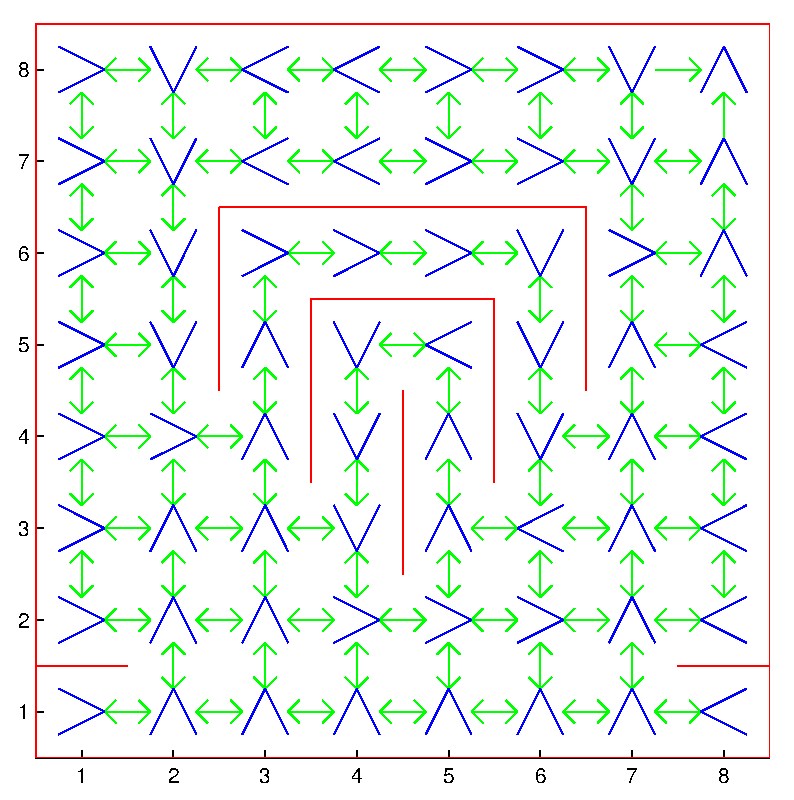
\includegraphics[width=0.5\textwidth]{StartingPolicy}\caption{Starting Policy and State Transitions}

\par\end{centering}

\end{figure}


\clearpage{}

\lstinputlisting[basicstyle={\scriptsize\ttfamily},breaklines=true,caption={part1.m},captionpos=b,commentstyle={\color{OliveGreen}},frame=tb,language=Matlab]{part1.m}


\subsection*{a) Policy Evaluation}

We represent state transition probabilities $\mathcal{P}_{ss'}^{a}$
as a MATLAB function which takes the current state and the action,
and returns a list of possible next states and a list of their probabilities.
We implement policy evaluation by stepping through these states in
a single-step backup, and repeat this until the change in the state
value function is sufficiently small. For the starting policy, our
evaluation converges after 23 steps. We implement policy improvement
by finding the greedy policy for the value function by searching in
each state for the action which maximises the expected return. Figure
2 shows the resulting value function and greedy policy.

\begin{figure}[H]
\centering{}\includegraphics[width=0.5\textwidth]{PolicyEvaluation}\caption{Value function and Greedy Policy}
\end{figure}


\medskip{}


\lstinputlisting[basicstyle={\scriptsize\ttfamily},breaklines=true,caption={part1a.m},captionpos=b,commentstyle={\color{OliveGreen}},frame=tb,language=Matlab]{part1a.m}


\subsection*{b) Policy Iteration}

We interleave policy evaluation and policy improvement until the policy
remains unchanged. This converges after 9 iterations of policy iteration.
The resulting policy by manual inspection seems to correctly take
the shortest path to the goal.

\begin{figure}[H]
\centering{}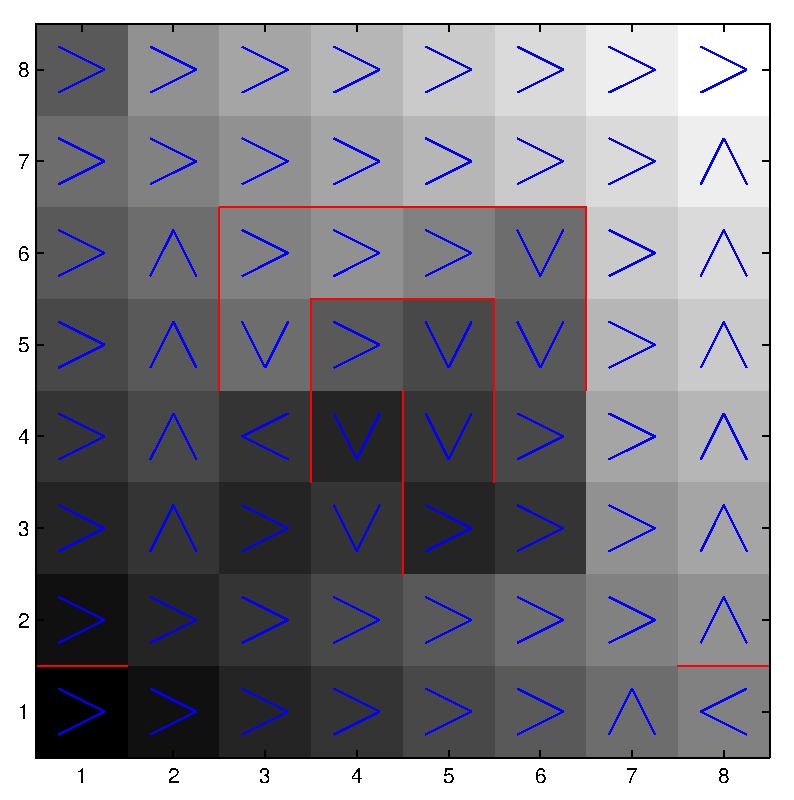
\includegraphics[width=0.5\textwidth]{NormalPolicyIteration}\caption{Optimal Value Function and Policy - Policy Iteration}
\end{figure}


\medskip{}


\lstinputlisting[basicstyle={\scriptsize\ttfamily},breaklines=true,caption={part1b.m},captionpos=b,commentstyle={\color{OliveGreen}},frame=tb,language=Matlab]{part1b.m}


\subsection*{c) Value Iteration}

We now use value iteration to directly compute the value of each state
as the value of the action which maximises the expected value of the
successor state. We repeat this until the value of each state remains
the same. This takes 15 iterations to converge. We compute the greedy
policy for the value function as before, this time only to visualise
it.

\begin{figure}[H]
\centering{}\includegraphics[width=0.5\textwidth]{NormalValueIteration}\caption{Optimal Value Function and Policy - Value Iteration}
\end{figure}


\medskip{}


\lstinputlisting[basicstyle={\scriptsize\ttfamily},breaklines=true,caption={part1c.m},captionpos=b,commentstyle={\color{OliveGreen}},frame=tb,language=Matlab]{part1c.m}


\subsection*{d) Sticky Walls}

We now introduce a sticky right wall. When in one of the states in
the rightmost column, there is a probability $p$ that we will stay
in the current state no matter which action was taken. We use a new
state transition function which returns the current state with probability
$p$, and run the previous policy iteration and value iteration code.
We start with $p=0.4$ and also compare with $p=0.6$. For states
next to the wall and far from the goal, it becomes worthwhile to step
away from the wall incurring a -1 penalty rather than try to stay
near the wall; even more so in the case where $p=0.6$. In the policy
iteration case, the number of policy iterations required for convergence
is still 9, but the value function requires up to 32 steps to converge
each iteration. In the value iteration case, the value function now
takes 52 iterations to converge, many more than the 15 seen previously.

\begin{figure}[H]
\centering{}\includegraphics[width=0.5\textwidth]{StickyPolicyIteration}\caption{Stick Walls - Policy Iteration}
\end{figure}
\begin{figure}[H]
\centering{}\includegraphics[width=0.5\textwidth]{StickyValueIteration}\caption{Stick Walls - Value Iteration}
\end{figure}
\begin{figure}[H]
\centering{}\includegraphics[width=0.5\textwidth]{StickyPolicyIteration6}\caption{Stick Walls - Policy Iteration, $p=0.6$}
\end{figure}


\medskip{}


\lstinputlisting[basicstyle={\scriptsize\ttfamily},breaklines=true,caption={part1d.m},captionpos=b,commentstyle={\color{OliveGreen}},frame=tb,language=Matlab]{part1d.m}\clearpage{}


\section{Secretary Problem}


\subsection*{a) MDP Design}

We specify the problem as an MDP as follows:

States: On step $K$, we have rejected the first $K-1$ applicants,
and we observe the ranking $R$ of the $K$th candidate relative to
them. There are $K$ such possible rankings, positions $1$ to $K$.
The rankings of the rejected candidates among themselves is irrelevant.
In MATLAB we represent these states in a triangular matrix. In the
MATLAB code we will represent the state by the values $K$ and $R$
and functions of those states as tables indexed by $K$ and $R$.

Terminal states: All states after the Accept action. We do not represent
these states explicitly in the MATLAB code.

Actions: Accept or Reject. On the 30th step we can only Accept. Represented
as $2$ and $1$ in the MATLAB code.

The total number of non-terminal states is $1+2+...+30=\frac{1}{2}N(N+1)=465$.

Reward: We assign to each candidate a random value $0-1$ according
to which they are ranked. The reward is the value of the accepted
candidate on entering the terminal state, $0$ otherwise.


\subsection*{b) Monte Carlo}

We simulate 25 million episodes. Each episode we generate random values
for the candidates and step through them in order. We use an $\epsilon$-greedy
on-policy monte-carlo algorithm with $\epsilon=0.1$.

Each step we insert our new candidate into a sorted list and thus
determine the candidate's rank. We take the action specified by the
$\epsilon$-greedy policy, and record the sequence of states we visit
in the episode. The sequence of $R$s visited and its length is sufficent
to determine the sequence of states and actions taken. At the end
of the episode, we use this list to update our estimate of $Q$ and
our greedy policy for the visited states. We compute the state-value
function $V$ from $Q$ for visualisation.

There is no strict convergence test for MC so we empirically detemined
25 million episodes as giving stable results. After 10 minutes of
computation we converge on the following policy, seen in Figure 8.
The white area indicates Accept actions. 1 is the highest rank. Right
at the start we always reject. A little later we will only accept
someone ranked very high. Right before the end, we will accept anyone
above average since on the final step we have to accept and expect
an average applicant value ($0.5$).

\begin{figure}[H]
\centering{}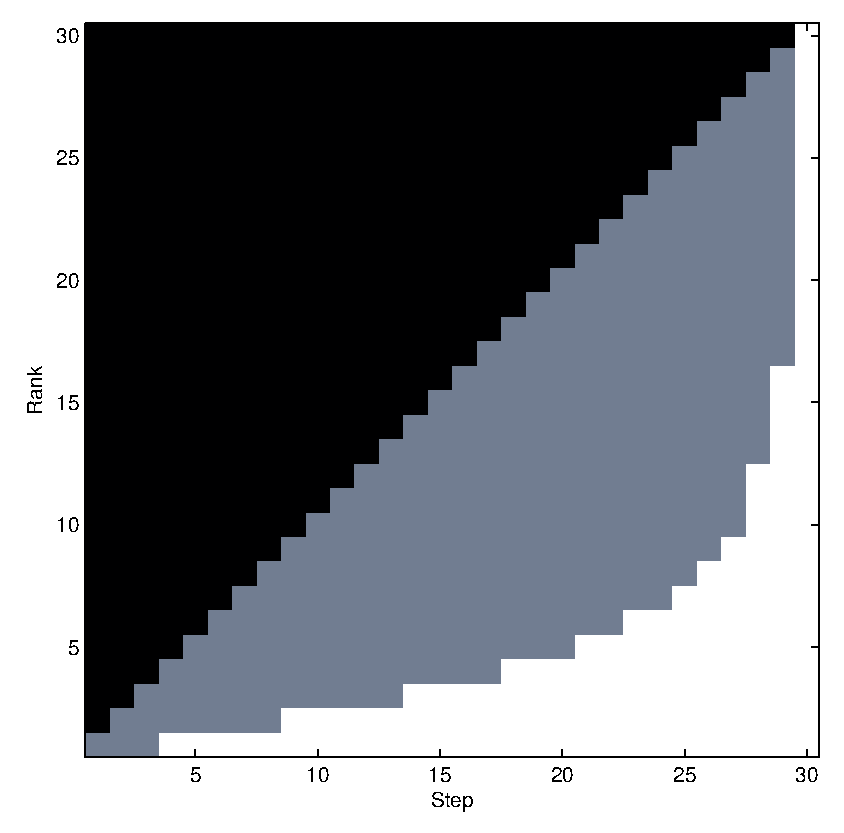
\includegraphics[width=0.5\textwidth]{SecretaryMDPPolicy}\caption{Policy after 25 million iterations}
\end{figure}
\begin{figure}[H]
\centering{}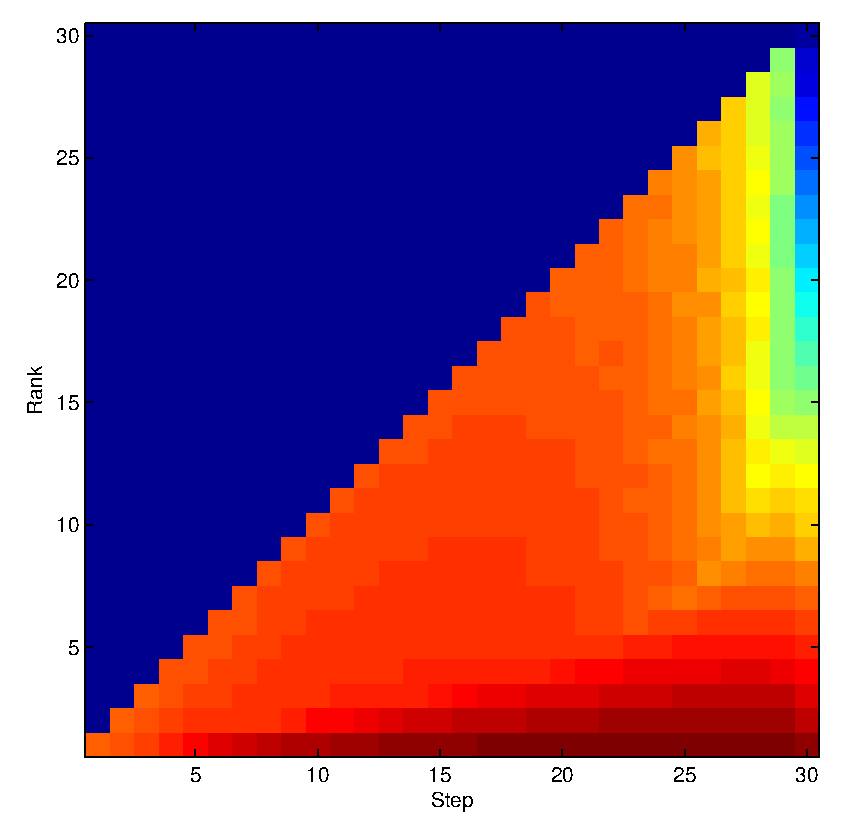
\includegraphics[width=0.5\textwidth]{SecretaryMDPVFunction}\caption{State value function after 25 million iterations}
\end{figure}
\medskip{}


\lstinputlisting[basicstyle={\scriptsize\ttfamily},breaklines=true,caption={part2b.m},captionpos=b,commentstyle={\color{OliveGreen}},frame=tb,language=Matlab]{part2b.m}


\subsection*{c) Q-Learning}

TODO


\section*{Appendix A - Additional Code}

\medskip{}
\lstinputlisting[basicstyle={\scriptsize\ttfamily},breaklines=true,caption={writeFigurePDF.m},captionpos=b,commentstyle={\color{OliveGreen}},frame=tb,language=Matlab]{writeFigurePDF.m}\medskip{}
\lstinputlisting[basicstyle={\scriptsize\ttfamily},breaklines=true,caption={makeLogFile.m},captionpos=b,commentstyle={\color{OliveGreen}},frame=tb,language=Matlab]{makeLogFile.m}
\end{document}
